\documentclass{beamer}

\usepackage{graphicx}
\setkeys{Gin}{width=\linewidth, height=0.8\textheight, keepaspectratio=true}
\usepackage[final]{movie15}
\usepackage[utf8]{inputenc}
\usetheme{WillBlack}

\title{El telescopio espacial Hubble}
\author
{
  William J. Henney
}                               %

\institute[CRyA, UNAM]
{
  Centro de Radioastronomía y Astrofísica\\
  UNAM, Morelia, México
}


\begin{document}

\begin{frame}
  \titlepage
\end{frame}

\begin{frame}
  \frametitle{El telescopio espacial Hubble}
  \includemovie[label=hubble-spin, autoplay, autopause, repeat]
  {\textwidth}{0.75\textwidth}{HST-telescope-rotate-high_quicktime.mov}
\end{frame}

\begin{frame}
  \frametitle{Datos rápidos}
  \begin{description}
  \item[Fecha de lanzamiento] 24 abril 1990
  \item[Costo inicial] \$1.5 mil millones USD
  \item[Costo a la fecha (1990--2012)] \(> \$10\) mil millones USD
  \item[Periodo de su órbita] 97 minutos
  \item[Datos científicos nuevos] 120 gigabytes por semana
  \end{description}
\end{frame}

\begin{frame}
  \frametitle{Los componentes del Hubble}
  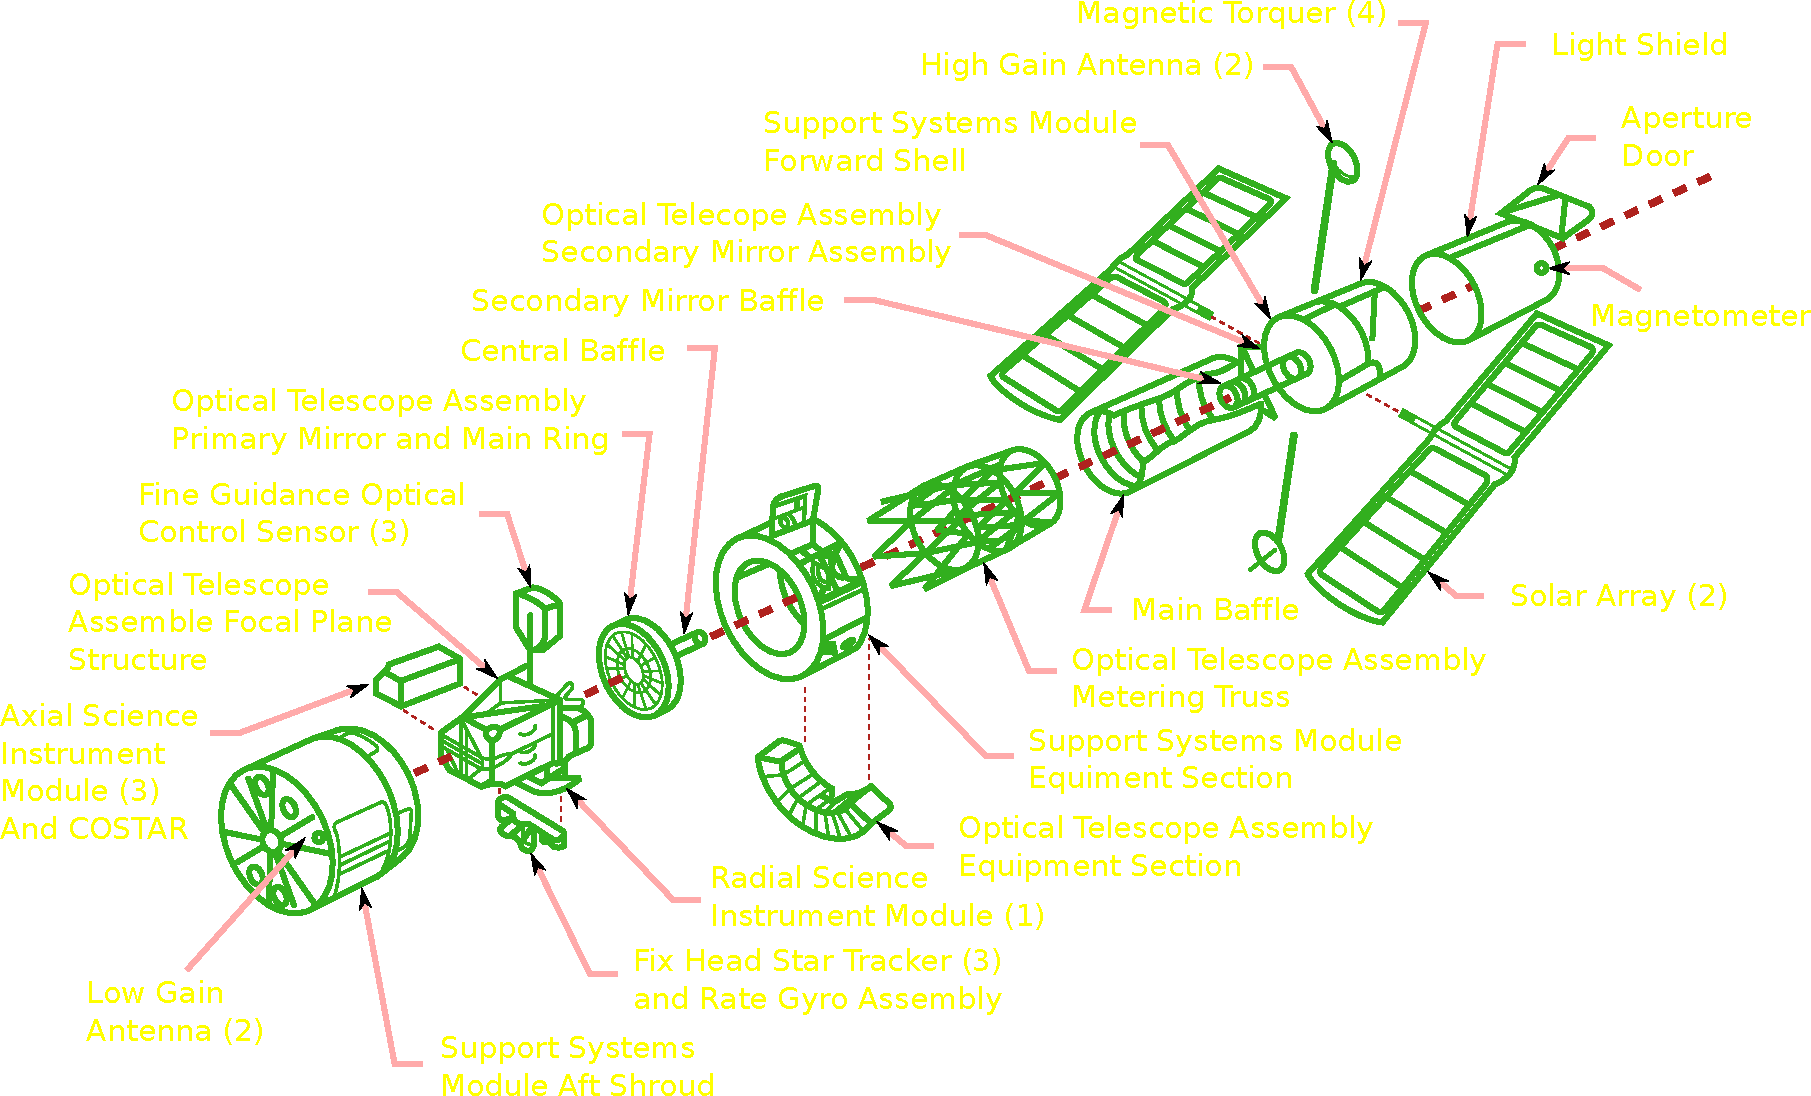
\includegraphics{HubbleExploded-lightBG}
\end{frame}

\begin{frame}
  \frametitle{El espejo primario}
  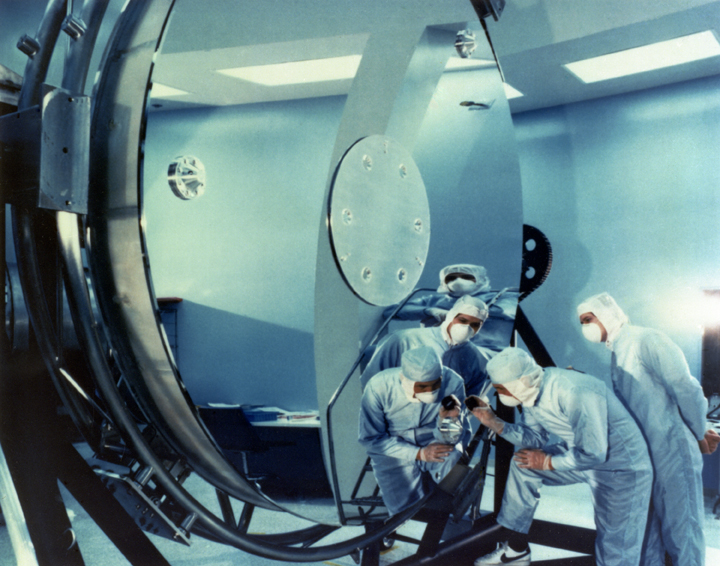
\includegraphics{hubble_mirror}
\end{frame}

\begin{frame}
  \frametitle{Los instrumentos -- cámaras}
  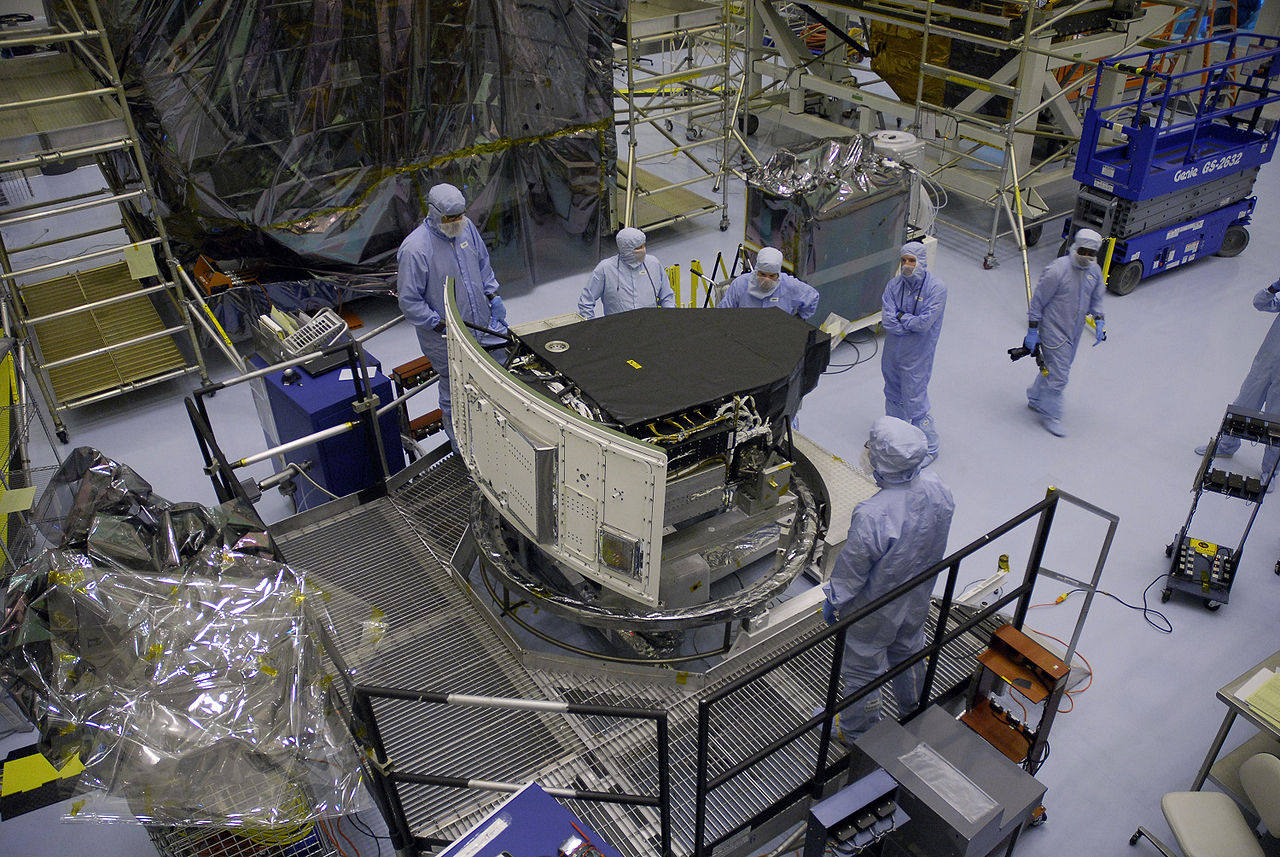
\includegraphics{1280px-Wide_Field_Camera_3}
\end{frame}

\begin{frame}
  \frametitle{Los instrumentos -- espectrógrafos}
  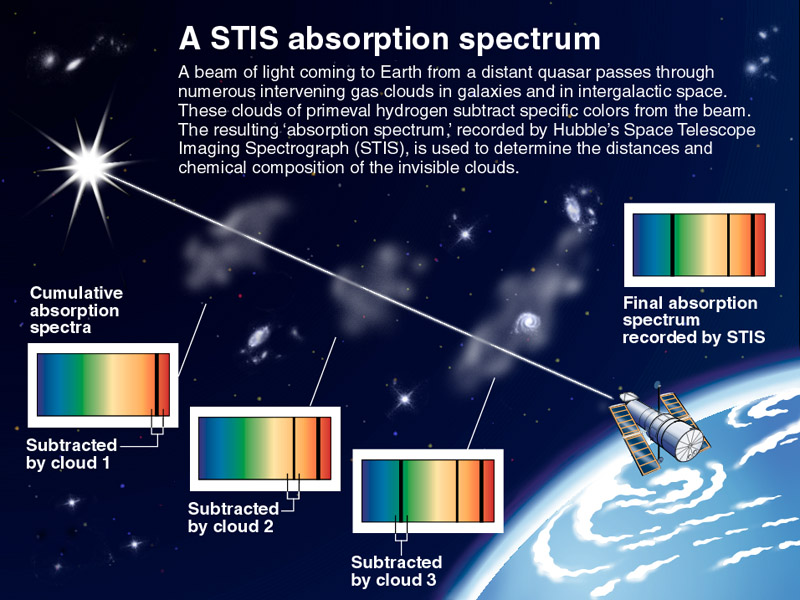
\includegraphics{STIS-absorption-spectrum}
\end{frame}

\begin{frame}
  \frametitle{Problemas iniciales -- Imágenes borrosas}
  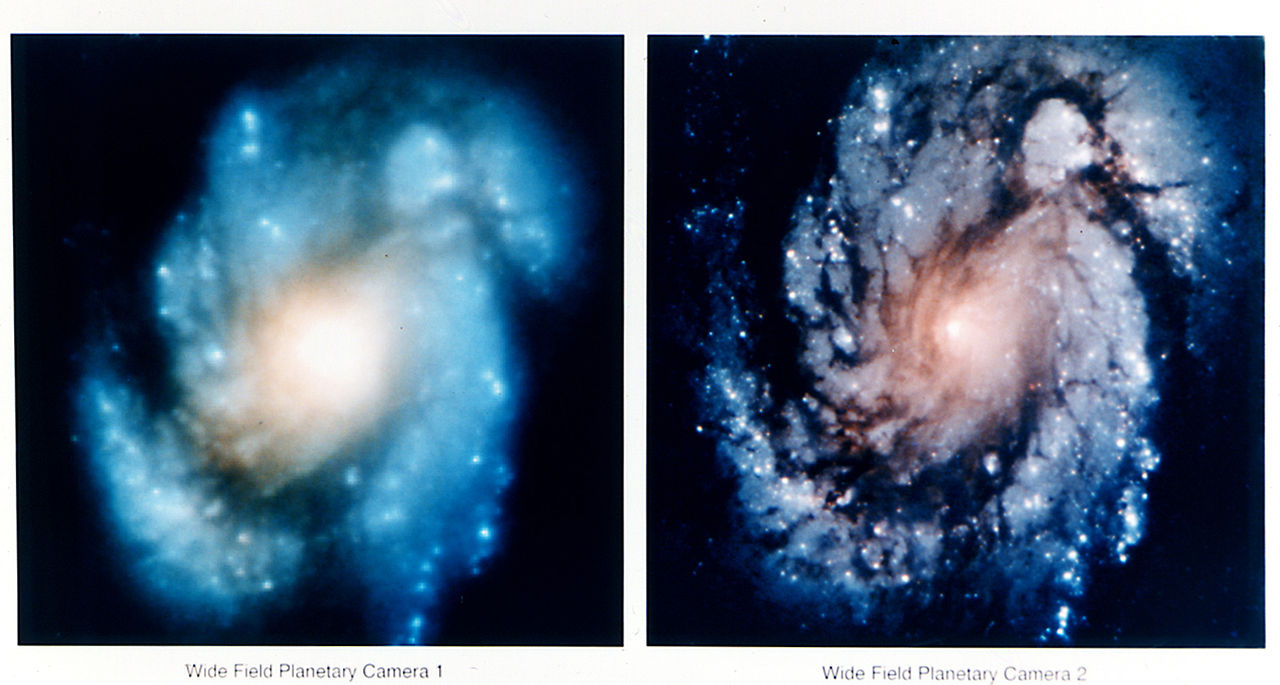
\includegraphics{1280px-Hubble_Images_of_M100_Before_and_After_Mirror_Repair_-_GPN-2002-000064}
\end{frame}

\begin{frame}
  \frametitle{Mantenimiento en órbita de los instrumentos}
  \includemovie[label=hubble-SM4, autoplay, autopause, repeat]
  {\textwidth}{0.5625\textwidth}{hst-sm4-short.avi}
\end{frame}

\begin{frame}
  \frametitle{Decubrimentos importantes: Formación Estelar}
  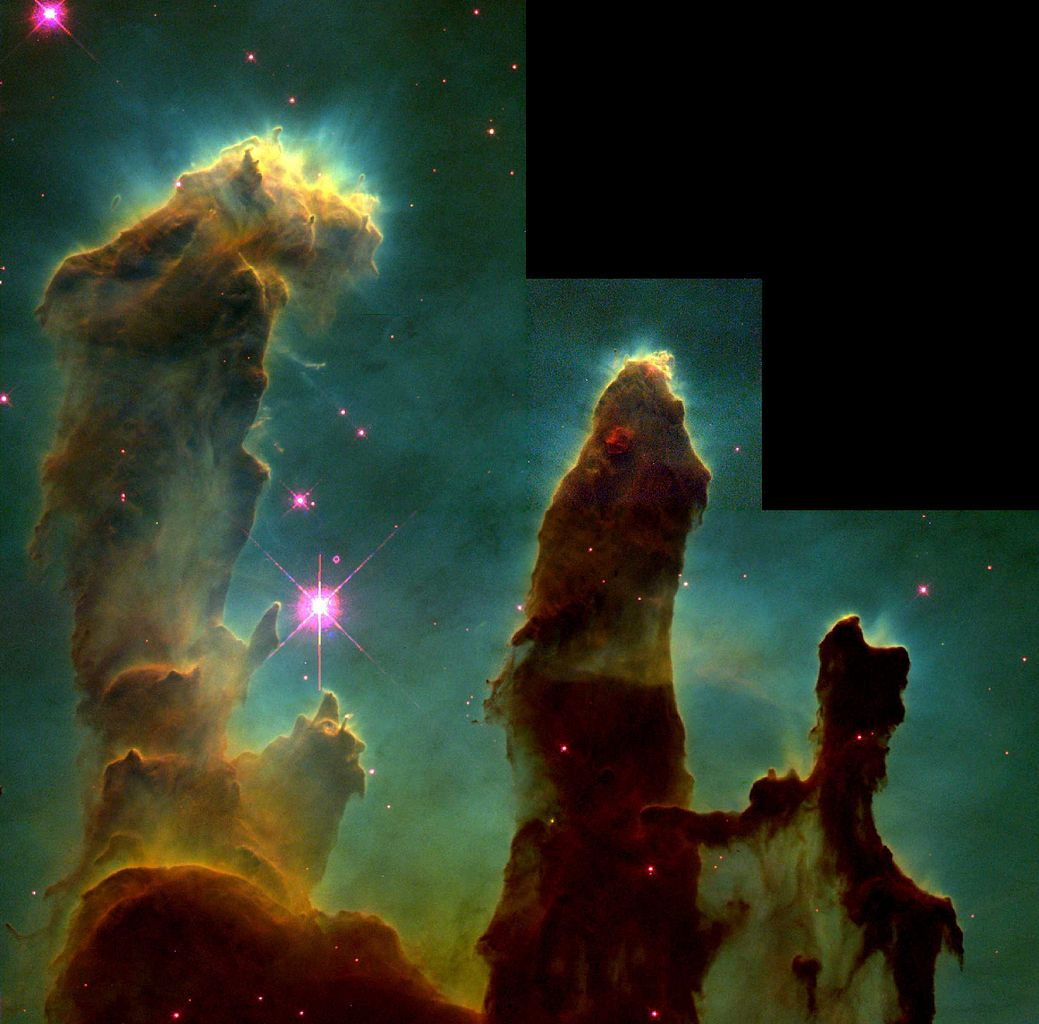
\includegraphics{1039px-Eagle_nebula_pillars}
\end{frame}

\begin{frame}
  \frametitle{Decubrimentos importantes: El Universo Temprano}
  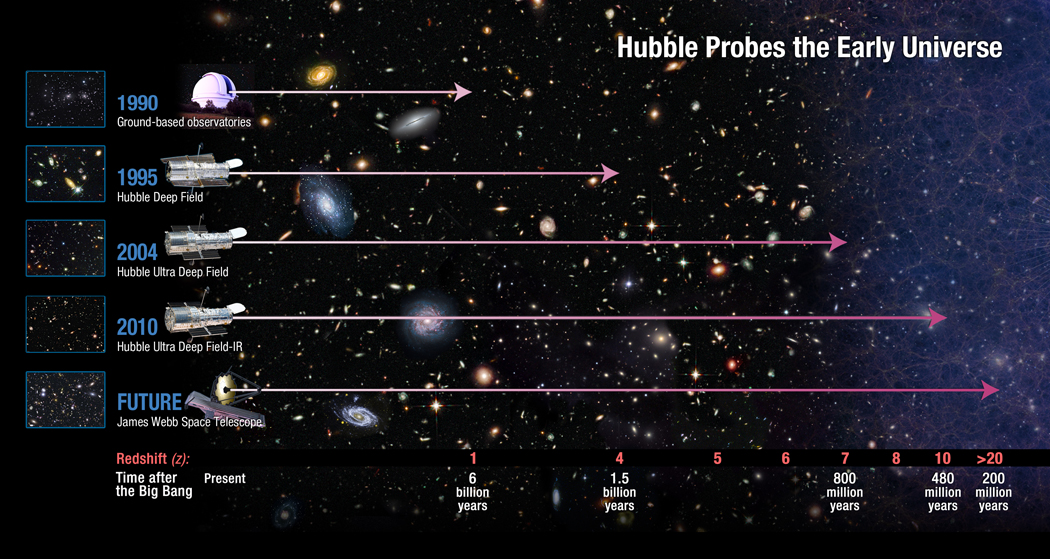
\includegraphics{hst-early-universe}
\end{frame}

\begin{frame}
  \frametitle{¿Cómo construimos las imágenes?}
  \includemovie[label=hubble-stitch, autoplay, autopause, repeat, palindrome]
  {0.8\textwidth}{0.545\textwidth}{hs-1995-45-a-low_mpeg.mpg}
\end{frame}

\begin{frame}
  \frametitle{¿Después del Hubble?}
  \begin{block}{James Webb Space Telescope}
    \begin{columns}\small
      \column{0.4\linewidth}
      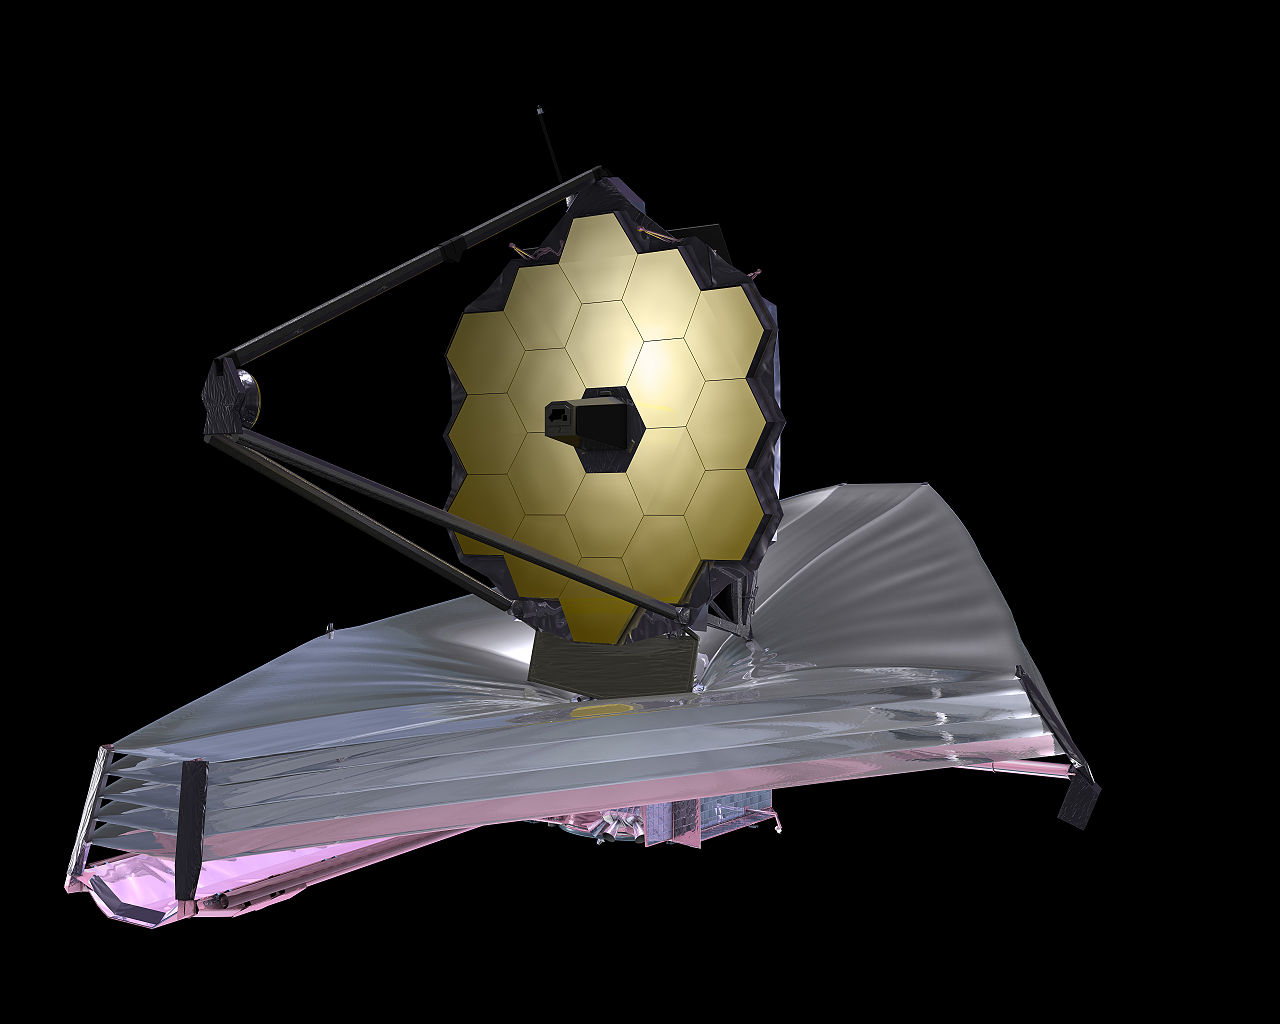
\includegraphics[width=1.5\linewidth]{1280px-James_Webb_Space_Telescope_2009_top}
      \column{0.6\linewidth}
      \begin{description}
      \item[Espejo] 6.5~m, segmentado
      \item[Órbita] Punto L2, 4 veces más lejos de la luna
      \item[Lanzamiento] ¿2018?
      \item[Costo] \$8.7 mil millones USD
      \end{description}
    \end{columns}
  \end{block}

\end{frame}

\end{document}
